\subsubsection{Uso por aficionado de los museos}

{\textbf {Resumen:}}
Un cliente habitual de los museos ve un folleto en la mesa principal de la entrada del museo, ve que hay una nueva App que permite ver el museo en su casa y que es interactivo, cuando vuelve a su casa, la descarga, imprime el código y empieza a descubrir cada una de las piezas del museo, fascinado con la aplicacion, comparte en redes sociales cada una de las piezas y el logro que obtuvo por completar el descubrimiento completo de las piezas de los museos regionales.

{\textbf {Actores:}}
Aficionado.

{\textbf {Propósito:}}
Evidenciar la conexión directa entre personas que frecuentas museos y la accesibilidad a la aplicación por parte de folletos dentro de los museos.

{\textbf {Referencias cruzadas:}}
R1.1, R1.2, R1.3, R1.4, R2.2, R2.3, R4.1, R4.2, R4.3, R4.4

\paragraph{Caso de Uso Esencial}

\begin{longtable}{|p{5cm}|p{8cm}|}
\hline 
Acción actores & Respuesta del sistema \\ 
\hline 
El usuario llega al lugar (museo) que contiene publicidad de la aplicación. & --- \\ 
\hline 
El usuario decide descargarla y utilizarla en su casa & --- \\ 
\hline
El usuario interactúa con la aplicación y descubre una pieza. & La aplicación da feedback de la pieza encontrada y muestra un botón para poder compartir directamente en redes sociales. \\ 
\hline
El usuario aprieta el botón para compartir en redes sociales. & Se despliega un panel con la información de la pieza para compartir y da la opción de que el usuario ingrese un mensaje personalizado. \\ 
\hline
El usuario escribe su mensaje y le da enviar. & El sistema  envía un formulario con la información pertinente a las redes sociales. \\ 
\hline
\caption{Tabla de Caso de Uso Esencial 1.6}
\label{tab26}
\end{longtable}

\paragraph{Diagrama de Caso de Uso}

\begin{figure}[H]
\centerline{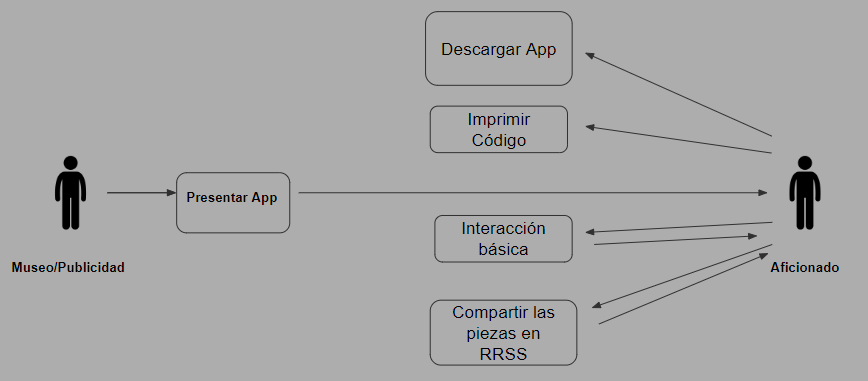
\includegraphics[width=15cm]{imgs/CasoUso_6.PNG}}
\caption{Diagrama Caso 1.6}
\label{fig_6_1}
\end{figure}

\paragraph{Modelo Conceptual}

\begin{figure}[H]
\centerline{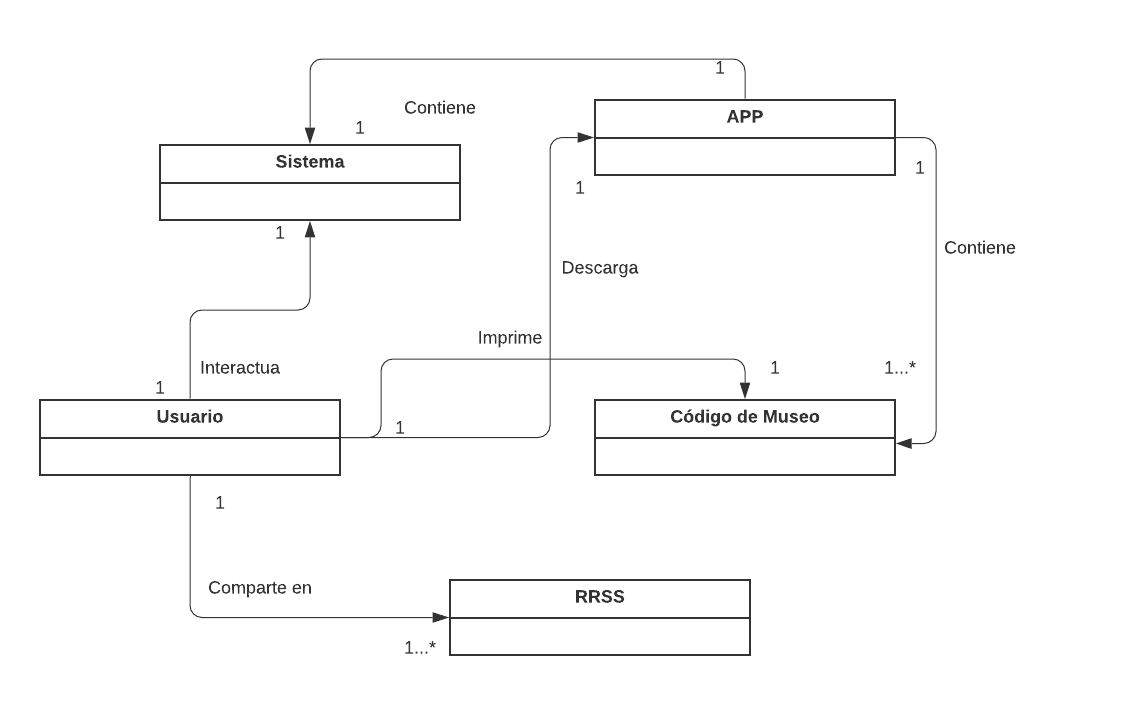
\includegraphics[width=15cm]{imgs/ModeloConceptualCaso_6_3.png}}
\caption{Modelo Conceptual Caso 1.6}
\label{fig_6_2}
\end{figure}

\paragraph{Diagrama de Secuencia o Colaboración}

\begin{figure}[H]
\centerline{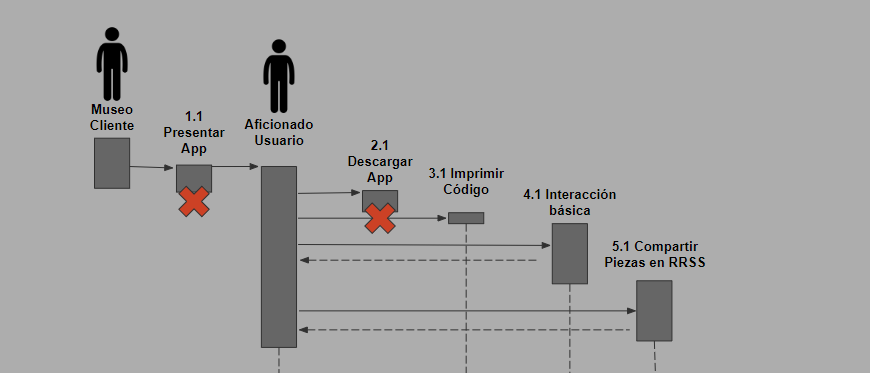
\includegraphics[width=15cm]{imgs/CasoUso_6_2.PNG}}
\caption{Diagrama de Secuencia Caso 1.6}
\label{fig_6_3}
\end{figure}

\paragraph{Priorización}
{\textbf {Tipo:}}
Principal.